\section{Experiments}
We run experiments on a dataset Study10 from University of Virginia on electricity disaggregation. 
This dataset collects data from 02/10/2014 to 02/21/2014, lasting for 12 days in a residential building. 
Both the two-phase aggregated data and each device's data are collected at an interval 2-3 seconds.
Totally 25 devices connect to two-phase at the entry of the house. 
Five of these devices are seldom operated, less than 5 times. 
Fourteen devices consume power less than 100W and majority of are lights. 
The largest power consumption of these devices is 11000W by heating indoor. 
The noise caused by device heatingIndoor is large, greater than 100W. 
Therefore we focus on disaggregation the six major electronic devices 
with power level larger than 100W. 
 
% the datasets from University of Virginia on both water and electricity disaggregation. 
%There are totally six data sets. The statistic of these six data set is listed in Table \ref{table_datasets}. 
%The recording interval of these datasets is 2 or 3 seconds. 
%A sensor is instrumented on each device to trace its ground truth operations. 
%\begin{table}[!t]
\renewcommand{\arraystretch}{1.3}
\caption{Electricity Dataset}
\label{table_datasets}
\centering
\begin{tabular}{|c|c|c|c|}
\hline
Data sets & Start date & End date & Duration (day) \\
\hline
\hline
Study 10 & 02-10-2014 & 02-21-2014 & 12\\
\hline
Study 11 & 01-27-2014 & 02-07-2014 & 12\\
\hline
Study 12 & 01-09-2014 & 01-21-2014 & 12\\
\hline
Study 13 & 12-23-2013 & 01-03-2014 & 12\\
\hline
Study 14 & 12-09-2013 & 12-20-2013 & 12\\
\hline
Study 101 & 06-09-2014 & 06-28-2014 & 20\\
\hline
\end{tabular}
\end{table}

\subsection{Electricity Disaggregation}
We assume that we know the power levels of each device. 
If the power levels of each device are unknown, 
we can use the sum of two-phase aggregated data and the on/off events of the 
ground truth to extract them. 
%In order to extract the power level of each device, 
We set a window size $w=30s$ ahead and behind of the ground truth events to match 
the aggregated data.
If there is only one power change in the aggregated data during these 60-seconds, 
this power level change must come from this event of a corresponding device. 
Usually, it takes around 2-5 seconds for an electrical device to reach
a steady power level state. 
The on and off events reflect different duration of a device to 
turn to a steady state. 
Therefore, we measure the minimal duration of the on event and off event 
of each device. 
After we go over all the aggregated data and ground truth on/off events, 
we run a Gaussian mixture model to the positive power changes and negative power changes
independently. The means and standard deviations correspond to  the on/off event of each device. 
The power levels, standard deviation, and on/off duration of each device of dataset study10 are listed in Table \ref{table_study10results}.
\begin{table*}[!t]
\renewcommand{\arraystretch}{1.3}
\caption{Power Levels, Standard Deviation of Power Levels, On/off Duration, Connected Phases and Disaggregation Results of Electricity Devices from Study10.}
\label{table_study10results}
\centering
%\small
\footnotesize
%\scriptsize
\setlength\tabcolsep{2pt}
\begin{tabular}{|c|c|c|c|c|c|c|c|c|c|c|}
\hline
\multirow{2}{*}{Device} & Power & Standard & On/off &  \multirow{2}{*}{Phase} & \multicolumn{3}{|c|}{Recursive Multivariate Motif Mining} & \multicolumn{3}{|c|}{AFAMAP}\\
\cline{6-11}
           &  Levels & Deviation & Duration &  &Precision&  Recall &  F-measure & Precision & Recall & F-measure\\ 
\hline
\hline
\multirow{2}{*}{HeatingIndoor+} & \multirow{2}{*}{10590W} & \multirow{2}{*}{1270W} & \multirow{2}{*}{60s} & \multirow{2}{*}{1+2} & \multirow{2}{*}{0.979} & \multirow{2}{*}{0.928} & \multirow{2}{*}{0.953} & \multirow{2}{*}{0.870}& \multirow{2}{*}{0.45} & \multirow{2}{*}{0.598}\\
HeatingOutdoor &  &  &  &  &  &  &  &  & & \\
\hline
Waterheater & 4450W & 350W &  2-5s & 1+2 & 0.999 & 0.997 &0.998 &0.627& 0.882 &0.733\\
\hline
Humidifier & 1470W & 90W & 10s & 1 & 0.997 & 0.992 &0.995 & 0.725 & 0.858 & 0.787\\
\hline
Microwave & 1850W & 200W & 10s & 2 & 0.95 &0.758 & 0.843 & 0.032 & 0.819 & 0.06\\
%\hline
%HeatingOutdoor & 4446W & 140 W & 2-18s & 1+2 &0.308 & 0.66& 0.42& & &\\
\hline
\multirow{2}{*}{Dryer} & 5200W &400W & 2-5s & 1+2 & \multirow{2}{*}{0.911}&\multirow{2}{*}{0.996}&\multirow{2}{*}{0.952}& \multirow{2}{*}{0.011}&\multirow{2}{*}{0.561} & \multirow{2}{*}{0.021}\\
\cline{2-3} \cline{4-5}
                       & 875W &225W  & 2-5s & 1 & & & & & &\\
%\hline
%L007 & 239W & 56W &  2-5s &2 & & & & & &\\
%\hline
%Fridge & 102W & 68W & 2-5s &1& - & - & - & & &\\
%\line
%L010 & 92W & 16W & 2-5s &2& & & & & &\\
%\cline
%L011 & 117W & 29W & 2-5s &1& & & & & &\\
%\hline
%L012 & 104W & 28W & 2-5s & 2& & & & & &\\
\hline
\end{tabular}
\end{table*}


%By analyzing each device, we notice that sometimes the power levels and 
%on/off duration are insufficient to identify the electric devices. 
%For instance, when the device heatingIndoor starts alone, 
%it takes $2-5$ seconds to go to a steady state as shown in Figure \ref{fig_heatingDevices} (a).
%But when the combined device of heatingIndoor and heatingOutdoor 
%starts, the starting duration takes around $4-18$ seconds. 
%In Figure \ref{fig_patterns} (b), after this combined device 
%starts for15 seconds, the power levels changes 
%for 9 times then to a relatively stable state. 
%During this period of 15 seconds, the power changes very rapidly. 
%If we accumulate these power levels together, 
%it's not a fix number. Therefore, for this kind of device, 
%we can only compare the shape of the startup to decide the on events 
%from the aggregated data. 

We apply recursive multivariate piecewise motif mining to dataset study10 
and compute the precision, recall and F-measure. 
Devices which draw power from both phases are separated first. 
They are heatingIndoor, waterheater and dryer.
\begin{figure*}[!t]
        \centering{
                \begin{tabular}{cc}
                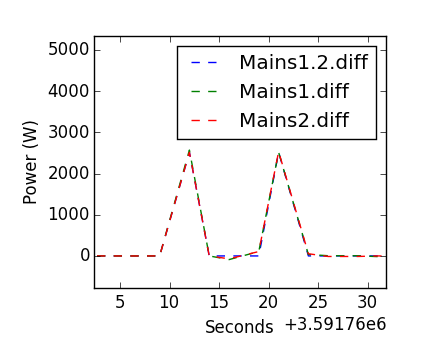
\includegraphics[width=3.2in]{multidisaggfig/heatingIndoorPhase12On.png} &
                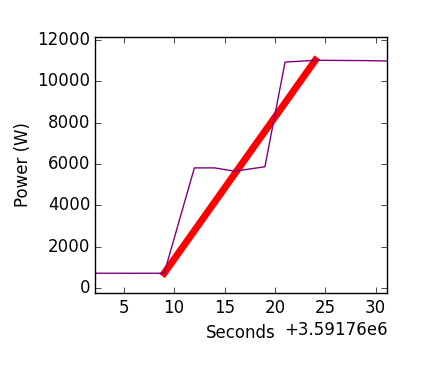
\includegraphics[width=3.2in]{multidisaggfig/heatingIndoorUp.png} &
                (a) & (b) \tabularnewline
                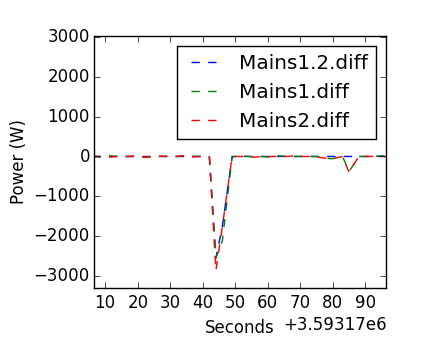
\includegraphics[width=3.2in]{multidisaggfig/heatingIndoorPhase12Off.png} &
                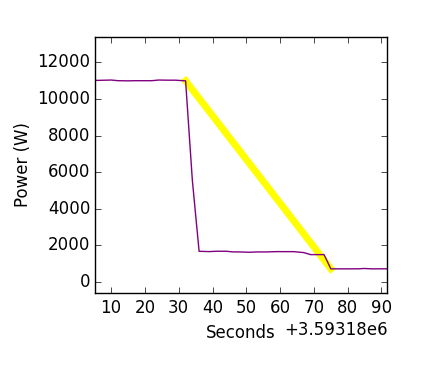
\includegraphics[width=3.2in]{multidisaggfig/heatingIndoorDown.png}\tabularnewline
                (c) & (d) \tabularnewline
                \end{tabular}
                }
        \caption{
        (a) On piecewise event and (c) Off piecewise event of heatingIndoor. heatingIndoor is disaggregated by motif mining the on event (b) and off event (d).}
        \label{fig_heatingIndoorResults}
\end{figure*}

Figure \ref{fig_heatingIndoorResults} (a) gives an example of 
on event in two-phase Mains1 and Mains2. 
Mains1.diff denotes the diffs data from Mains1 and Mains2.diff represents 
the diffs data from Mains2. 
Mains1.2.diff marks blue when Mains1 and Mains2 share the similar power changes. 
We can see that 
the power consumption of a specific device jumps twice in two-phase simultaneously.
At the first time, both phases jump 2572W. After nine seconds, 
the power of both phases increase  2520W. 
The sum of these four changes is 10184W. 
Comparing with the power levels of all devices, 
we speculate that these power changes are caused 
by device heatingIndoor. 
%By applying multivariate piecewise motif mining, 
%we match the power consumption with $11000W$ and 
%categorize this on event into heating indoor. 
Figure \ref{fig_heatingIndoorResults} (b) shares the same snippet in time series as Figure \ref{fig_heatingIndoorResults} (a). 
The red line indicate that the on event of heatingIndoor is recognized.    
\begin{figure*}[!t]
        \centering{
                \begin{tabular}{cccc}
                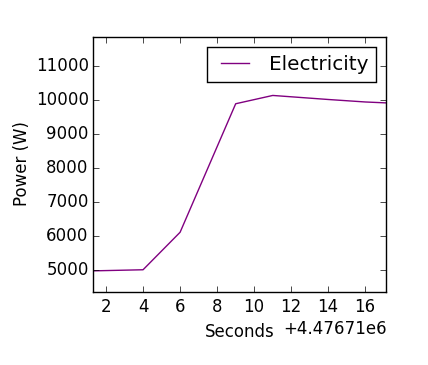
\includegraphics[width=3.2in]{multidisaggfig/dryerPhase_sum.png} &
                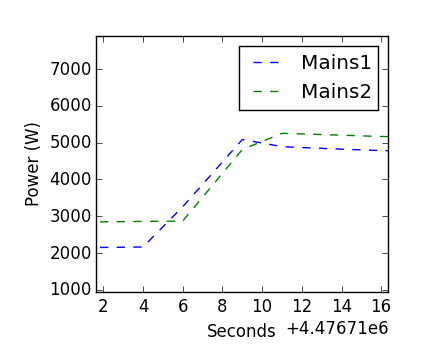
\includegraphics[width=3.2in]{multidisaggfig/dryerPhase12On.png} \tabularnewline
                (a) & (b) \tabularnewline
                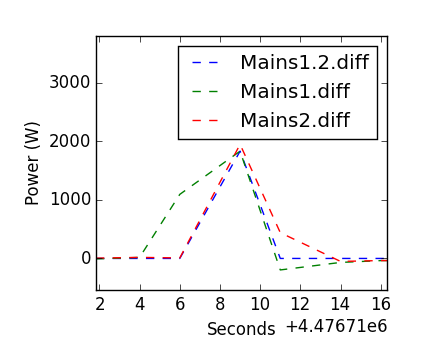
\includegraphics[width=3.2in]{multidisaggfig/dryerPhase12OnDiff.png} &
                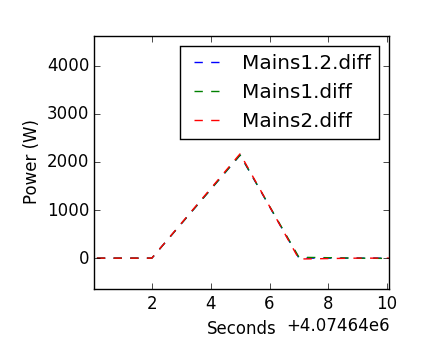
\includegraphics[width=3.2in]{multidisaggfig/waterHeaterPhase12OnDiff.png}\tabularnewline
                (c) &(d) \tabularnewline
                \end{tabular}
                }
        \caption{
        Disaggregating dryer with multivariate motif mining.
        (a) the startup in the sum of aggregated power (b) the startup in two phases (c) the diffs in two phases on event of dryer.
        (d) the diffs in two phases on event of water heater which shares same power level as dryer but different patterns when drawing power from two-phases.
        }
        \label{fig_dryerResults}
\end{figure*}

Similarly, the off event plunges twice in two seconds -2877W and -1759W in both phases as shown in Figure \ref{fig_heatingIndoorResults} (c).
The sum of this off event is -9272W. 
After matching the power levels, we categorize it as the off event of heatingIndoor Figure \ref{fig_heatingIndoorResults} (d). 

Dryer shares the same power level with waterheater at around 4800W. 
If disaggregating these two devices from the sum of two phases, 
it's hard to distinguish them. 
But with multivariate piecewise motif mining, these two devices 
are distinguished. 

Figure \ref{fig_dryerResults} (a) and (b) shows the on event of dryer from sum of phase 1 and phase 2, 
and these two phases separately. 
From \ref{fig_dryerResults} (c) and (d) are the diffs data of dryer and waterheater. 
We can see that waterheater draws power from phase 1 and phase at the same time. 
But dryer shows a different pattern. It draws power from phase 1 at a lower power 1093W then jumps to 1830W.
and at the same time, it draws power from phase 2 jumping to 1946W directly. 
We encode them as shown in Figure \ref{fig_eventEncoding} then apply motif mining to disaggregate them. 
 
After deleting the power consumption from both aggregated phases, 
we apply piecewise motif mining again to single phase. 
Then we discover devices humidifier from phase 1 
and device microwave from phase 2. 
%Note that the power consumption of humidifier and microwave overlaps sometimes, 
%which makes it hard to separate them. 
%But they draw power from different phases separately. 
%Multivariate motif mining can separate them. 
When we only disaggregate with the sum of phase 1 and phase 2, 
the precision recall result on microwave and humidifier is not so good 
because sometimes their power consumptions are similar. 
But with multivariate motif mining, we can separate them very clearly 
with good precision and recall. 
The precision and recall results on the data set study10 are listed in Table \ref{table_study10results}.

Recursive multivariate motif mining is capable of disaggregating continuous variable load. 
\begin{figure*}[!t]
        \centering{
                \begin{tabular}{cccc}
                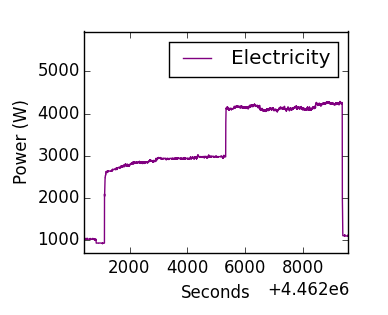
\includegraphics[width=3.2in]{multidisaggfig/heatingIndoorOutdoorPattern1_sum.png} &
                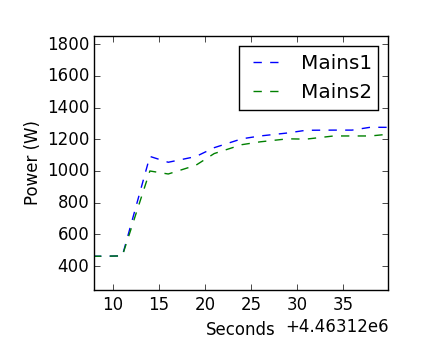
\includegraphics[width=3.2in]{multidisaggfig/heatingIndoorOutdoorPattern1.png} \tabularnewline
                 (a) & (b)\tabularnewline
                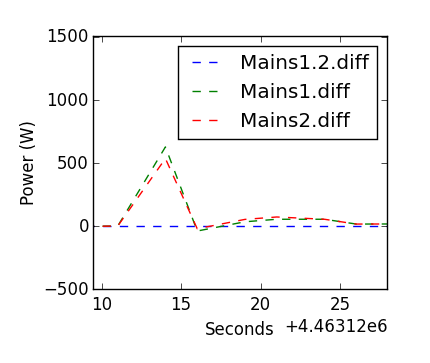
\includegraphics[width=3.2in]{multidisaggfig/heatingIndoorOutdoorPhase12On_1.png} &
                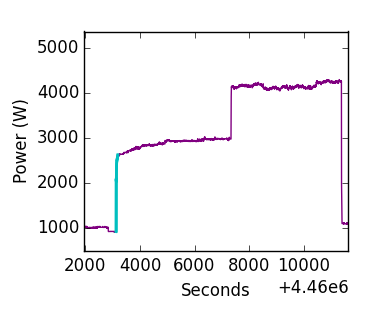
\includegraphics[width=3.2in]{multidisaggfig/heatingIndoorOutdoorFittedPattern1.png}\tabularnewline
                (c) &(d) \tabularnewline
                \end{tabular}
                }
        \caption{
        Disaggregating continuous variable load heating outdoor. 
        (a) the startup in the sum of aggregated power (b) the startup in two phases (c) the diffs in two phases (d) the disaggregated on event of heating outdoor.}
        \label{fig_heatingOutdoorResults}
\end{figure*}

Figure \ref{fig_heatingOutdoorResults} (a) illustrates the startup of heatingOutdoor.
During this on event, its power levels change for 9 times then to a relatively stable state as shown in 
Figure \ref{fig_heatingOutdoorResults} (b) and (c). 
By applying piecewise motif mining, 
we can successfully identify this heatingOutdoor device 
after matching its power level. 
The disaggregated result is displayed in Figure \ref{fig_heatingOutdoorResults}.
Note that this continuous variable load startup snippet can be discovered by dynamic time warping 
subsequence search as well if this device is on without the intervene of other devices.
If another device  $D$ which draws from phase 1 or phase 2 is turned on or off during this period, 
multivariate piece-wise motif mining can still identify this heatingOutdoor device. 
The reason is that $D$ only uses on phase's power, 
its power change is Not counted in our piecewise event. 
